\documentclass{article}

\usepackage{amsmath}
\usepackage{graphicx}
\usepackage{subcaption}


\author{Kalman Joseph Szenes}
\title{HPCSE2: Exercise 2}

\begin{document}
    \maketitle

    \section{Task 1}

    \begin{figure}[ht]
        \begin{subfigure}[b]{0.5\linewidth}
            \centering
            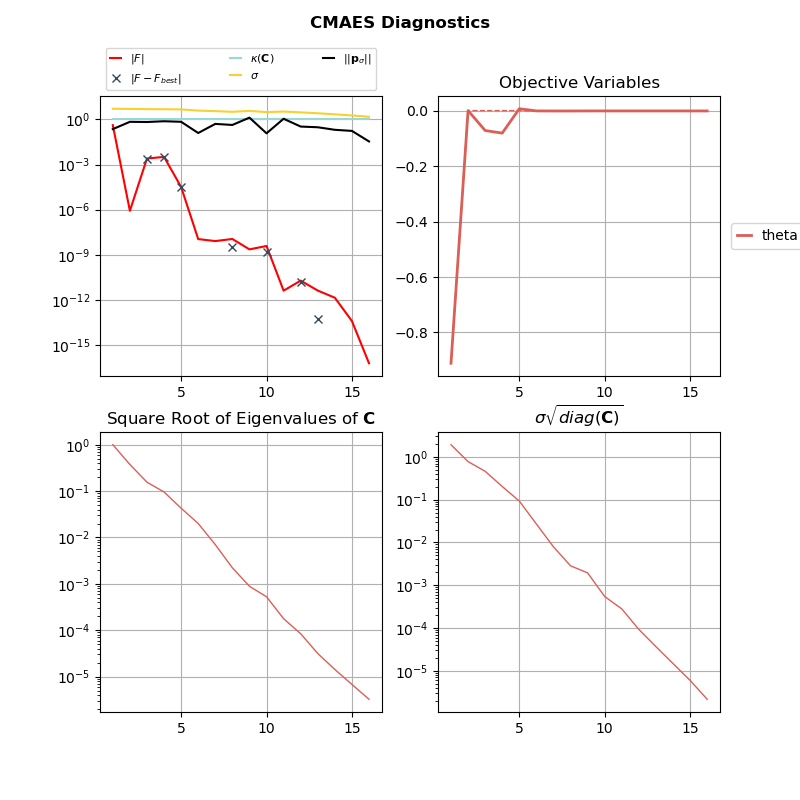
\includegraphics[width=0.95\linewidth]{img/example_1.png}
        \end{subfigure}
        \begin{subfigure}[b]{0.5\linewidth}
            \centering
            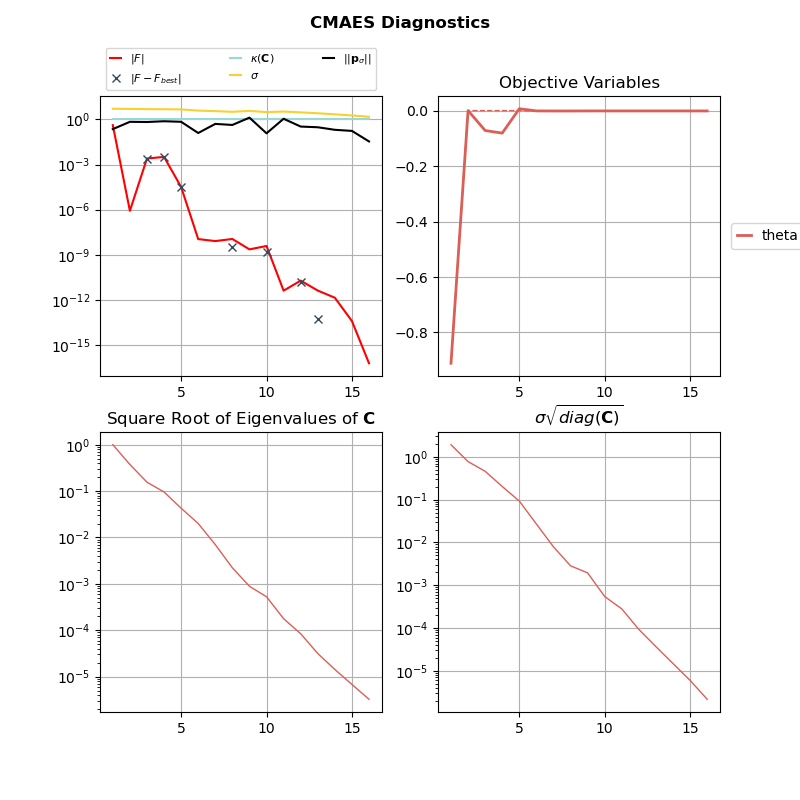
\includegraphics[width=0.95\linewidth]{img/example_1.png}
        \end{subfigure}
        \begin{subfigure}[b]{0.5\linewidth}
            \centering
            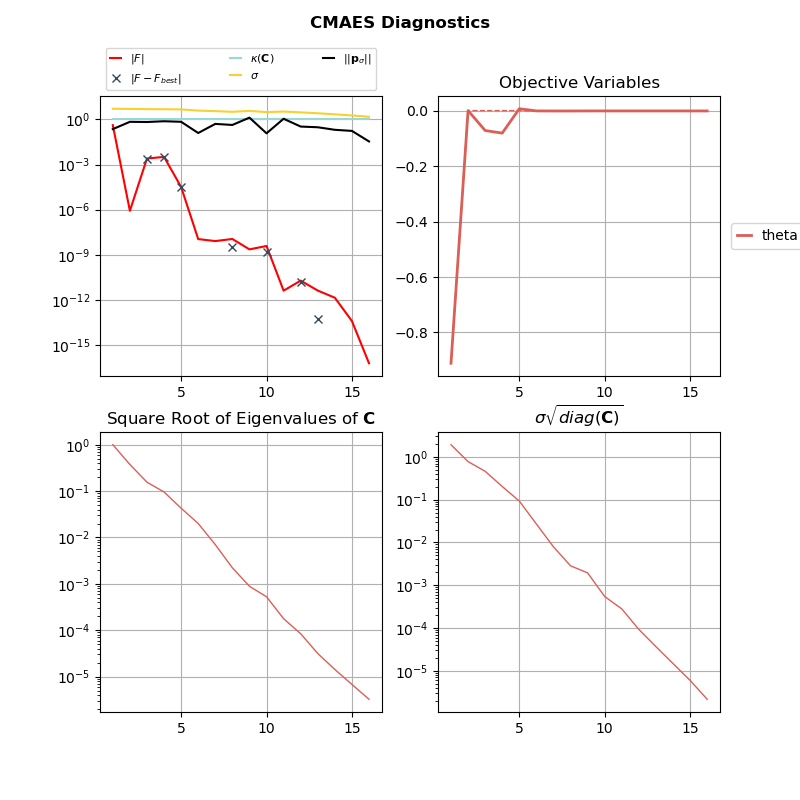
\includegraphics[width=0.95\linewidth]{img/example_1.png}
            \caption{Example 3}
        \end{subfigure}
        \caption{Plots showing Korali output for Example 1, 2 and 3 of Task 1.}
    \end{figure}

    \section{Task 2}
    \begin{figure}
        \centering
        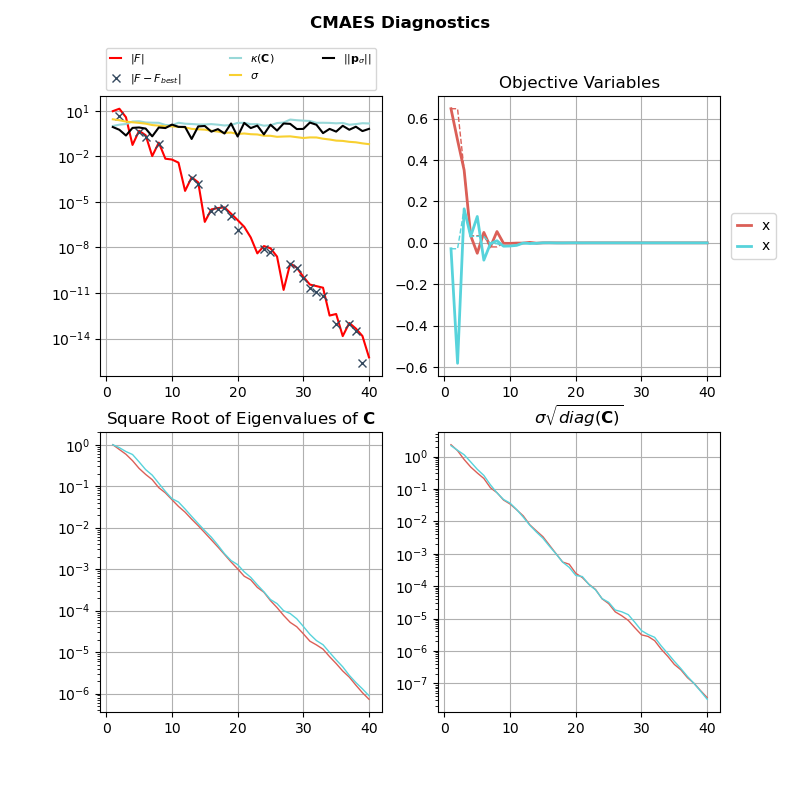
\includegraphics[width=0.7\textwidth]{img/task2.png}
        \caption{Plot showing Korali output for Task 2.}
    \end{figure}
    Korali finds the following minimum at $(x_{min}, y_{min})$ = $(-4.219e-09, +2.051e-09)$ with $f(x_{min}, y_{min}) = -5.721571e-16$. This is reaching the value 0.0 with machine precision.
    This solution is trivial as all terms in f are squared and hence the minimum is found at the origin with value 0.

    When the optimization was run with different number of samples, we observed negative correlation with the number of generation. Hence, if we increase the number of samples, the number of generations decreases.

    \section{Task 3}
    Bayesian inference can be used for parameter approximation technique and it relies on Bayes' Theorem:
        
    \begin{align}
        P(\theta | data) &= \frac{P(data | \theta) P(\theta)}{P(data)}
        \label{eq:1}
    \end{align}

    In this equation, $\theta$ groups together all the parameters that we would like to approximate.

    In Bayesian inference, our prior probability distribution of the parameters ($P(\theta)$) is updated and improved as we obtain more data.
    The prior represents our best guess for the probability distribution of the parameters before observing the data.
    In the agnostic case, we simply assign to it a Uniform distribution in a reasonable range (i.e. $P(\theta) \sim U[\theta_{min}, \theta_{max}]$).
    The prior is multiplied by a likelihood function ($P(data|\theta)$) which represents the probability of obtaining the observed data give the parameters.
    We assign to it the parametrised model with which we would like to describe the data. 
    For this problem, as we assume that there is an error in the measured data, we will model the likelihood using a normal distribution with a mean given by our assumed model ($P(data | \theta) \sim N(k_1 x + k_3 x^3 + k_5 x^5, \sigma^2)$).
    Finally, to ensure that our posteriori is well behaved, we need to normalise the numerator by the appropriate factor ($P(data) = \int_{\theta} P(data | \theta) P(\theta) d\theta$ which is called the evidence.
    In Bayesian inference, this factor is not important, as we want to find the maximum a posteriori with respect to the parameters. Since the evidence does not depend on the parameters and is hence simply a constant, it will not affect the maximum.


    In this concrete case, equation \ref{eq:1} can be written:

    \begin{equation}
        P(\theta | data) \sim N(k_1 x + k_3 x^3 + k_5 x^5, \sigma^2) * U[\theta_{min}, \theta_{max}]
    \end{equation}

    We chose as range [-5, 5] for the parameters and [0, 5] for the standard deviation.
    We can find the maximum by taking the derivative with respect to the parameters and setting it to zero.
    We would then need to make sure that the stationnary point obtained is maximum not a minimum.


    \begin{figure}[htb]
        \begin{subfigure}[b]{0.5\linewidth}
            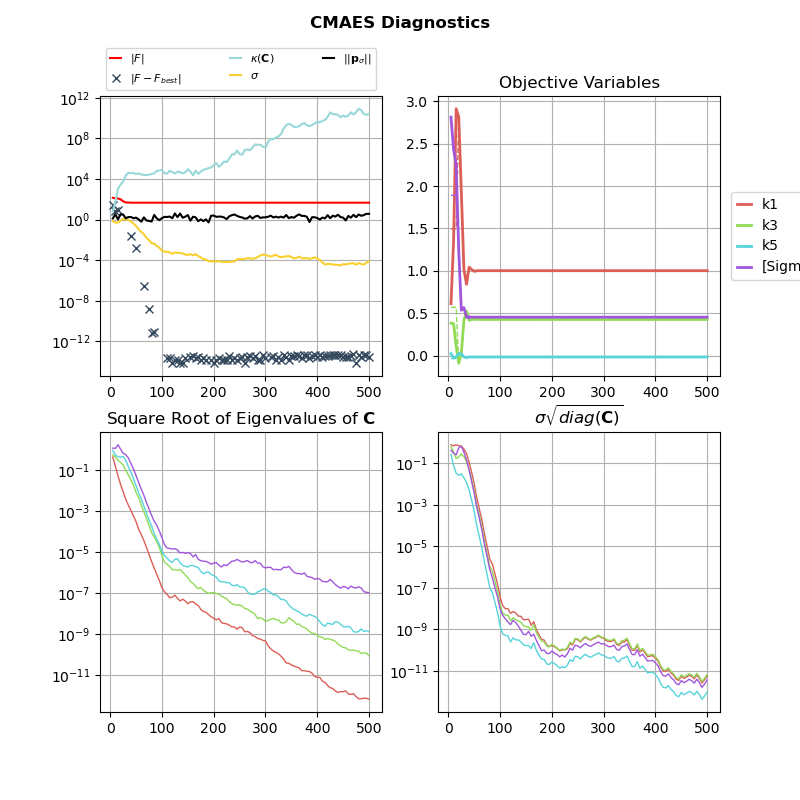
\includegraphics[width=0.95\linewidth]{img/task3_b.png}
            \caption{CMA-ES optimization.}
        \end{subfigure}
        \begin{subfigure}[b]{0.5\linewidth}
            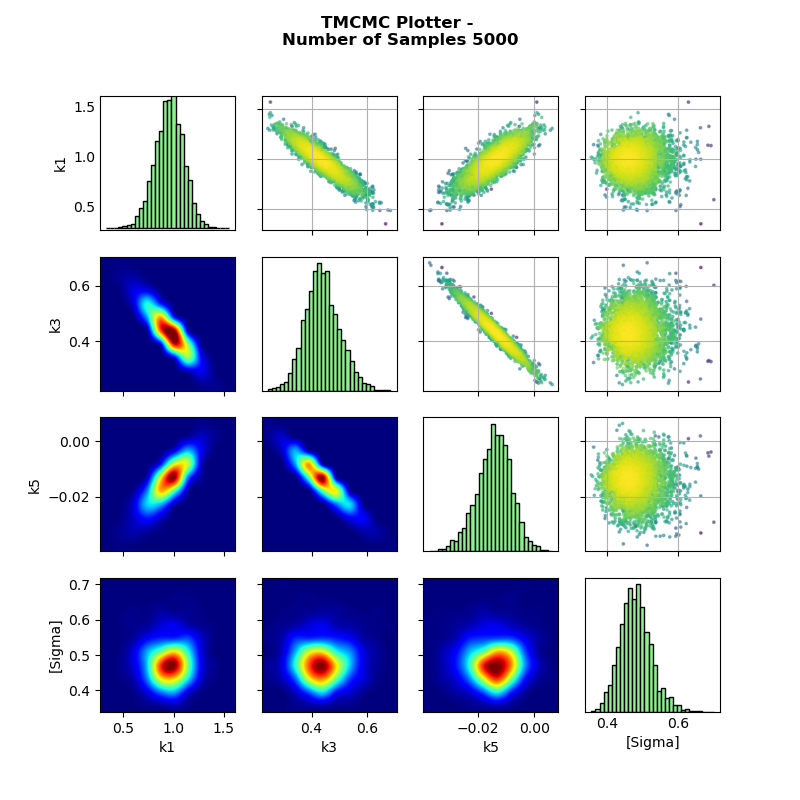
\includegraphics[width=0.95\linewidth]{img/task3_c.png}
            \caption{TMCMC optimization.}
        \end{subfigure}%%

        \begin{subfigure}[b]{0.5\linewidth}
            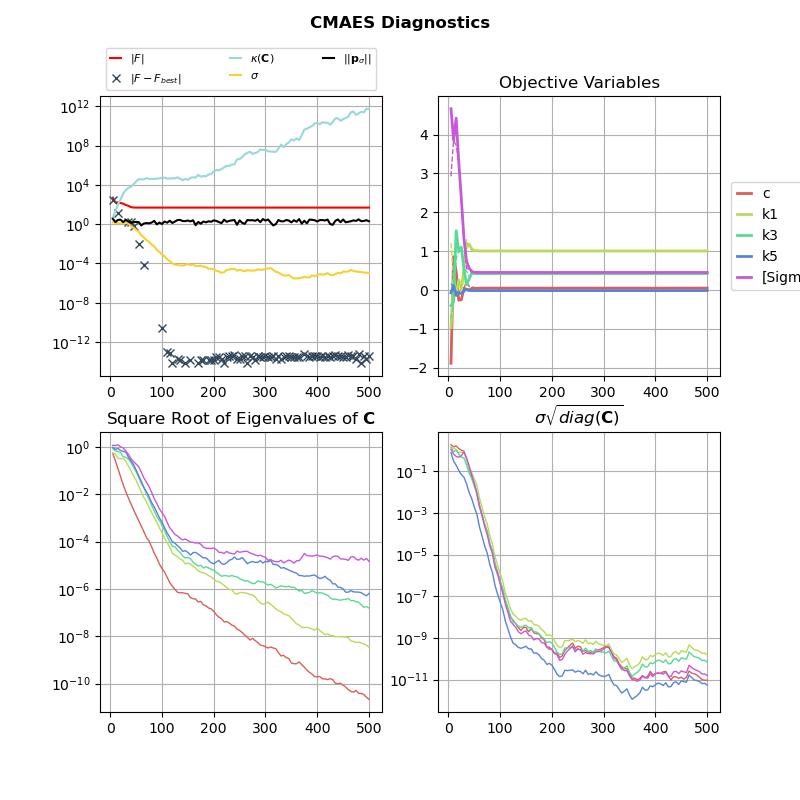
\includegraphics[width=0.95\linewidth]{img/task3_d_cmaes.png}
            \caption{CMA-ES optimization with offset.}
        \end{subfigure}
        \begin{subfigure}[b]{0.5\linewidth}
            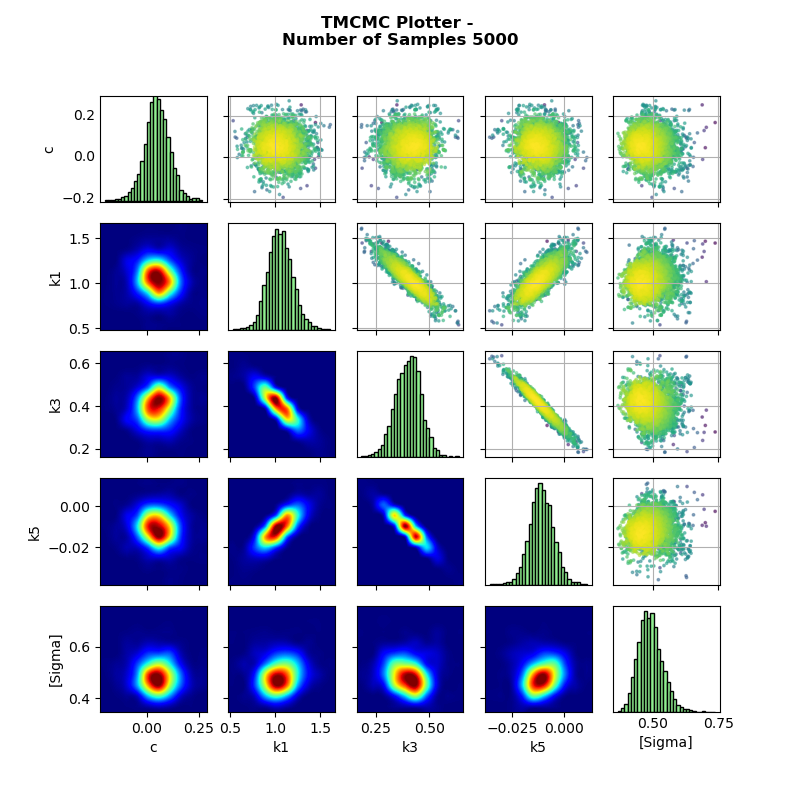
\includegraphics[width=0.95\linewidth]{img/task3_d.png}
            \caption{TMCMC optimization with offset.}
        \end{subfigure}

        \caption{Plots for Task 3.}
        \label{fig:task3}
        
    \end{figure}

    As illustrated in Figure \ref{fig:task3} (a), the maximum likelihood exhibits smooth convergence for all the parameters

    As illustrated in Figure \ref{fig:task3} (b), k1 and k5 are negatively correlated with k3 and k5 is positively correlated with k3. The standard deviation does not seem to be correlated with the other parameters.

    As illustrated in Figure \ref{fig:task3} (c), the maximum likelhood converges smoothly with the added offset as well. However, as illustrated in Figure \ref{fig:task3} (d), adding the offset does not seem to significantly decrease the correlation between the other parameters.
    It is hence preferable to use a simpler model (without offset).




\end{document}